\textbf{Chapter 1: Introduction}
\begin{center}
    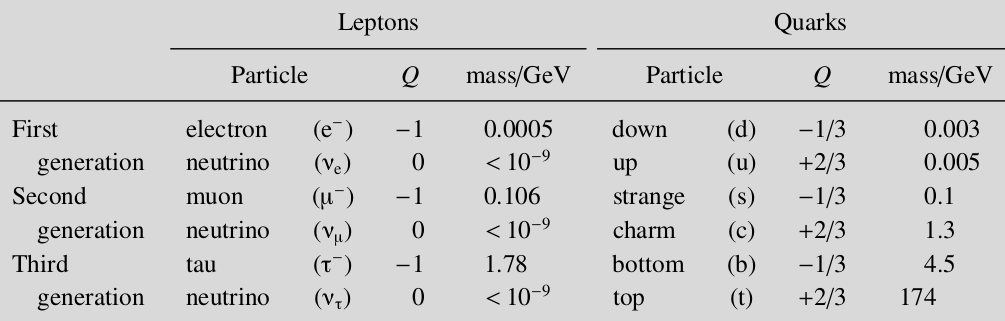
\includegraphics[width=\linewidth]{images/quark_info.png}
    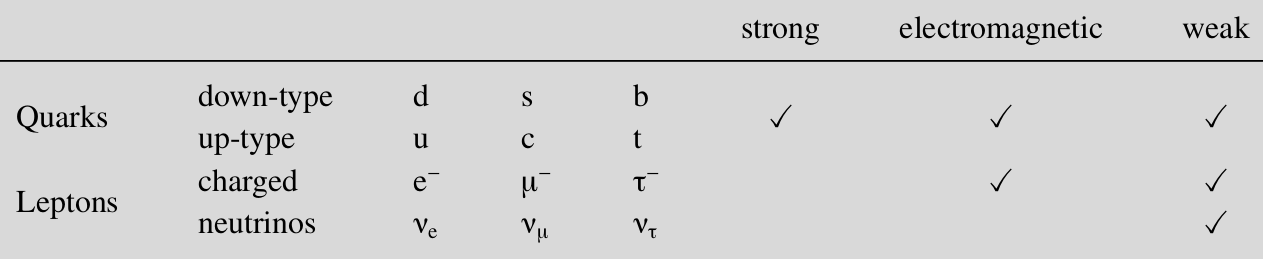
\includegraphics[width=\linewidth]{images/which_forces_for_which_particles.png}
    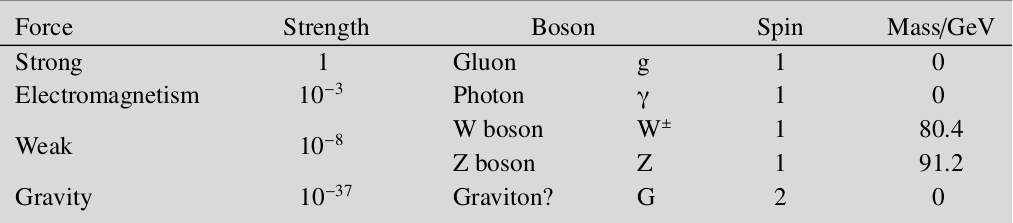
\includegraphics[width=\linewidth]{images/boson_info.png}
    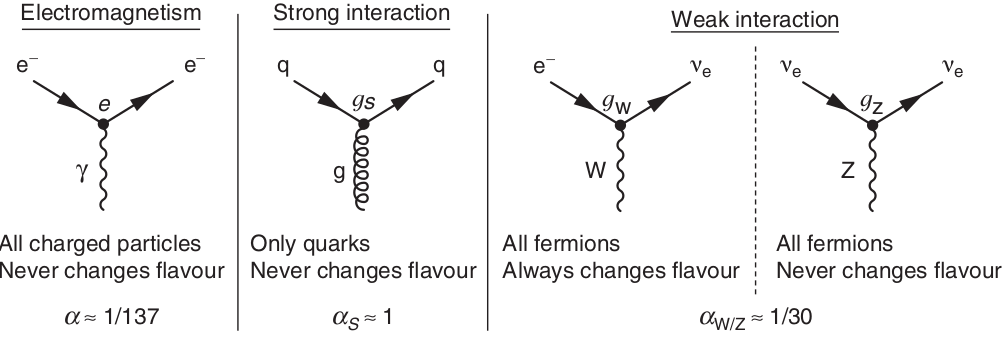
\includegraphics[width=\linewidth]{images/interaction_basics.png}
\end{center}
Bethe-Bloch:
\begin{align*}
    \frac{dE}{dx} &\approx -4\pi\hbar^2 c^2 \alpha^2 \frac{nZ}{m_2v^2}\left(\ln\left(\frac{2\beta^2\gamma^2c^2m_e}{I_e}\right) - \beta^2\right)\\
    v &= \beta c, n = \text{num dens}, Z=\text{atom num}, I_e \approx 10Z\text{eV}, \alpha = 1/137
\end{align*}
Detectors:
\todo[inline]{More about detector types?}
Mag field tracking: $p\cos(\lambda) = 0.3BR$

Cerenkov: $\cos(\theta) = \frac{1}{n\beta}$

After x rad. lengths $\expval{E} = \frac{E}{2^x}$. $x_{\text{max}}$
\begin{center}
    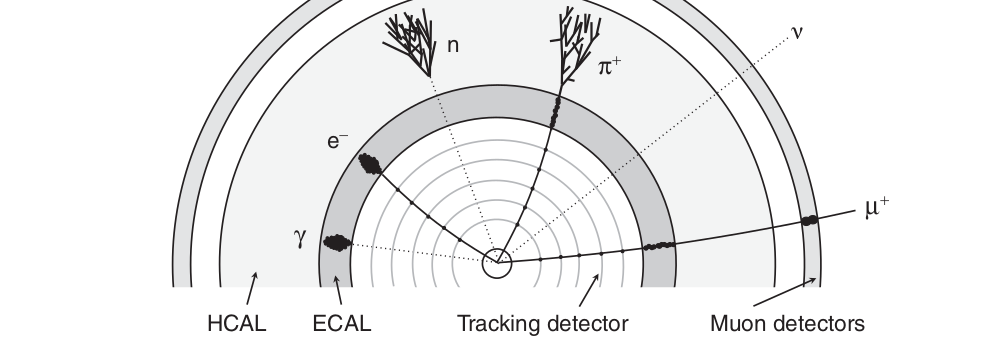
\includegraphics[width=\linewidth]{images/particle_tracks.png}
\end{center}
B-tagging: look for secondary vertices

Number of events and cross sections: $N = \sigma\int \mathcal{L}(t)dt$

In 2 colliding bunches, $\mathcal{L} = f(\SI{}{Hz}) \frac{n_1 n_2}{4\pi \sigma_x \sigma_y}$
